Com a finalidade de validar a interface, foi contruído e simulado um ambiente \textit{indoor} mostrado na Figura%~\ref{fg:ambiente}.\\
. Nele foram feitas medições(sempre com a porta fechada). Os objetos presentes durante esse processo, tais como bancadas, divisória de vidro, monitores e gabinetes foram considerados na modelagem.\\

Alguns desse objetos estão dispostos em alturas diferentes em relação ao piso. As bancadas e o teto estão a uma altura de 0,75 metros e 2,73 metros, respectivamente.\\

Como resultado da modelagem usando a interface, obeteve-se a estrutura mostrada na Figura(colocar figura estrutura da interface). A disposição dos seus objetos seguiu a posicionamento real dos mesmos na hora em que foram feitas medições.
%\begin{figure}[ht!]
%	\centering
%	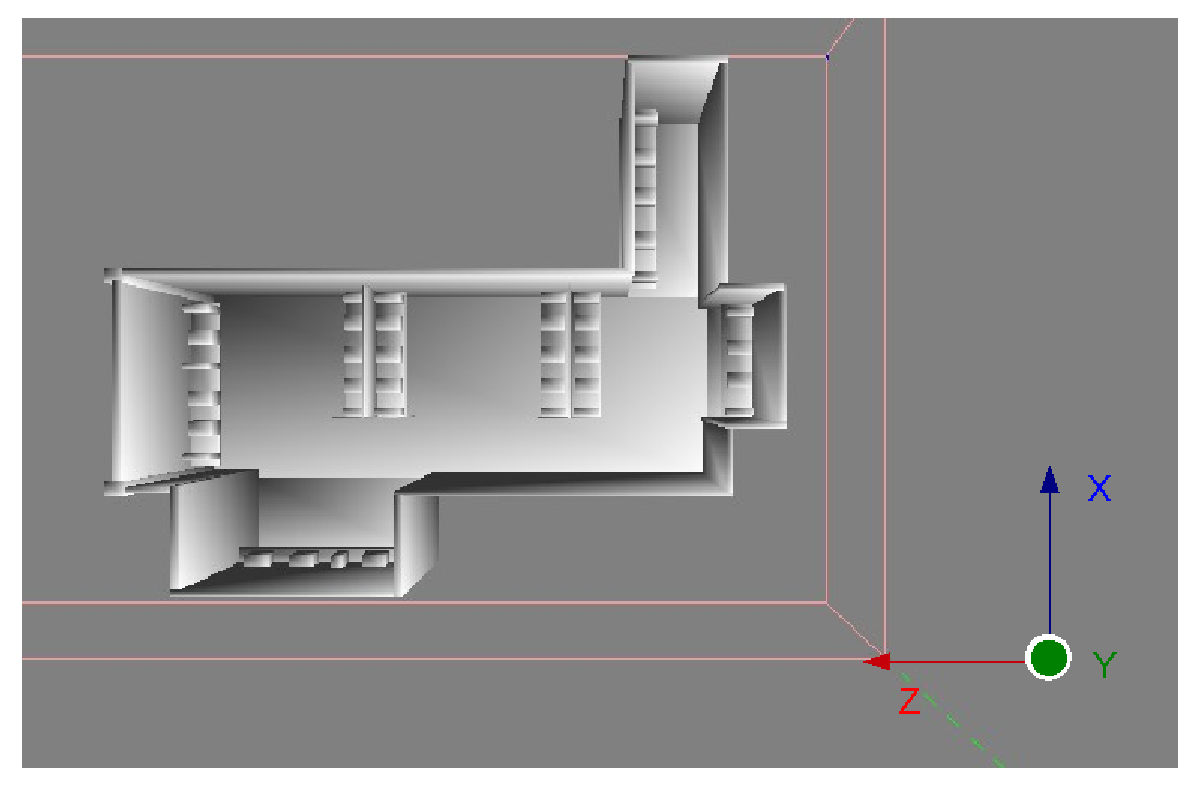
\includegraphics[scale = 0.4]{ambiente}
%	\caption{Visão topo em pespectiva do ambiente construído através da interface.}
%	\label{fg:ambiente}
%\end{figure}

As especificações desse cenário, foram:
\begin{itemize}
	\item \textit{Delta}(Tamanho da célula de Yee) utilizada foi de $0,003m$.
	\item \textit{Região de Análise} com dimensões: $X$ = $15m$, $Y$ = $3m$ e $Z$ = $15m$.
	\item \textit A lista das carateristicas físicas com seus respectivos matérias estam presentes na Tabela~\ref{materiais}
\end{itemize}

\begin{center}
\begin{tabular}{|l|l|l|l||l|}
%\label{materias}
	\hline
	Elementos dos Ambiente & Material & $\epsilon$ & $\sigma$ & $\mu$ \\ \hline
	Parede & Tijolo & 4 & 0,0135 & 1\\ \hline
	Teto & Gesso & 2,8 & 0,1533 & 1 \\ \hline
	Bancadas & Madeira & 1,8 & 0,011 & 1\\ \hline
	Monitores e Gabinetes & Metal & 5 & $valor$ & 1\\ \hline
	Divisórias & Vidro & 5 & $valor$ & 1 \\ \hline
	Piso & Concreto & 5 & 1 & 1 \\
	\hline
\end{tabular}
\label{materiais}
\end{center}

%antena
Depois de ambiente ter sido montado, surguiu a necessidade de se introduzir uma antena. Como a que foi usada na medição não tinha uma representação virtual, foi necessário criá-la. Com isso foram feitos alguns teste usando antenas dipolo, com o intuito de obeter a máxima aproximação do comportamento da antena real. O primeiro deles foi utilizando os paramentros mostrados na Figura(colocar antena 1).\\

Foi utilizada em todos os teste uma fonte de tensão de trem de pulsos normalizado, Figura~\ref{fg:fonte}, onde através da transforma de Fourier, pode-se observar se essa fonte estava trabalhando na banda adequada. O resultado obtido foi o ilustrado na Figura~\ref{fg:fonte_f}.\\
\begin{figure}[ht!]
	\centering
	\includegraphics[scale = 0.4]{fonte}
	\caption{Gráfico da fonte(trêm de pulsos).}
	\label{fg:fonte}
\end{figure}
\begin{figure}[ht!]
	\centering
	\includegraphics[scale = 0.4]{fonte_f}
	\caption{Gráfico da fonte transformada de Fourier da fonte.}
	\label{fg:fonte_f}
\end{figure}
 Visto que o sua perda de retorno não foi satisfatória, foram feitas modificações em sua dimensão e por fim foi adicionado um  capacitor(Figura(colocar figura antena capacitor)). Com essas mudanças se obteve um antena com um comportamento parecido com o da real. Os gráficos de perda dessas duas construções esta ilustrado na Figura~\ref{fg:perda}.  





%resultados
